\chapter{METODOLOGIA DE LA INVESTIGACION}

\section{Enfoque de la investigación}

La presente investigación tiene un enfoque cuantitativo y experimental, ya que se busca generar un dataset que sirva como entrada para el entrenamiento de un modelo de detección de objetos (YOLOv8) y evaluar su desempeño en la identificación de equipos de protección personal (EPP), específicamente cascos de seguridad, en un entorno de obra real. El enfoque cuantitativo se justifica por la medición de variables como la precisión del modelo y la calidad de las imágenes procesadas, mientras que el enfoque experimental se debe a la implementación y prueba de diferentes algoritmos de corte y técnicas de preprocesamiento de imágenes.

\section{Diseño de la Investigación}

El diseño de la investigación es no experimental, ya que no se manipularán directamente las variables independientes (el uso de cascos de seguridad por parte de los trabajadores). En su lugar, se recolectarán datos a través de la captura de imágenes reales en una obra de construcción, y se procesarán mediante técnicas de visión por computadora. Este diseño incluye un trabajo de campo para la recolección de datos (imágenes de los trabajadores) y un trabajo de laboratorio para el procesamiento, etiquetado y análisis del dataset.

\section{Recolección de Datos}

\subsection{Selección del Sitio de Estudio}

La obra seleccionada para la toma de imágenes es el proyecto denominado ``COMERCIO''. Se eligió este entorno porque refleja condiciones reales de trabajo en construcción, donde los trabajadores utilizan equipos de protección personal, incluyendo cascos de seguridad. Se solicitó previamente el permiso necesario para acceder a la obra y realizar la toma de fotografías sin interferir con las actividades de la obra.

La obra esta ubicada en la region de Arequipa, en el distrito de Cono Norte, Asentamiento Poblacional Asociacion de Pequenos Industriales y Artesanos Arequipa APPIAR Mz N Lotes 1.

\begin{figure}[!ht]
  \centering
  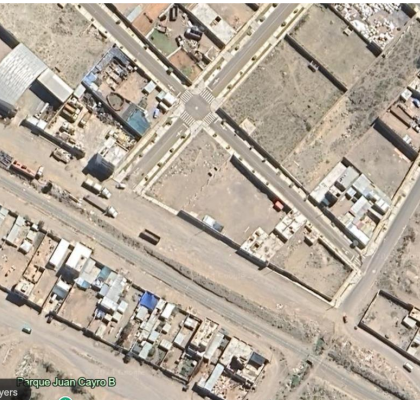
\includegraphics[width=.49\linewidth]{images/comercio.png}
  \caption{Ubicacion referencial de la obra ``Comercio''.}
  \label{fig:comercio}
\end{figure}

\subsection{Equipamiento Utilizado}

Para la captura de las imágenes, se utilizó un dispositivo móvil de la maraca Honor X8a \ref{fig:honor} con sistema operativo Android, con una cámara que permite obtener fotografías de alta resolución con dimensiones de 5992x4344 píxeles. Este equipo fue seleccionado por su facilidad de uso y su disponibilidad para capturar imágenes de manera espontánea en el entorno de la obra.

\begin{figure}[!ht]
  \centering
  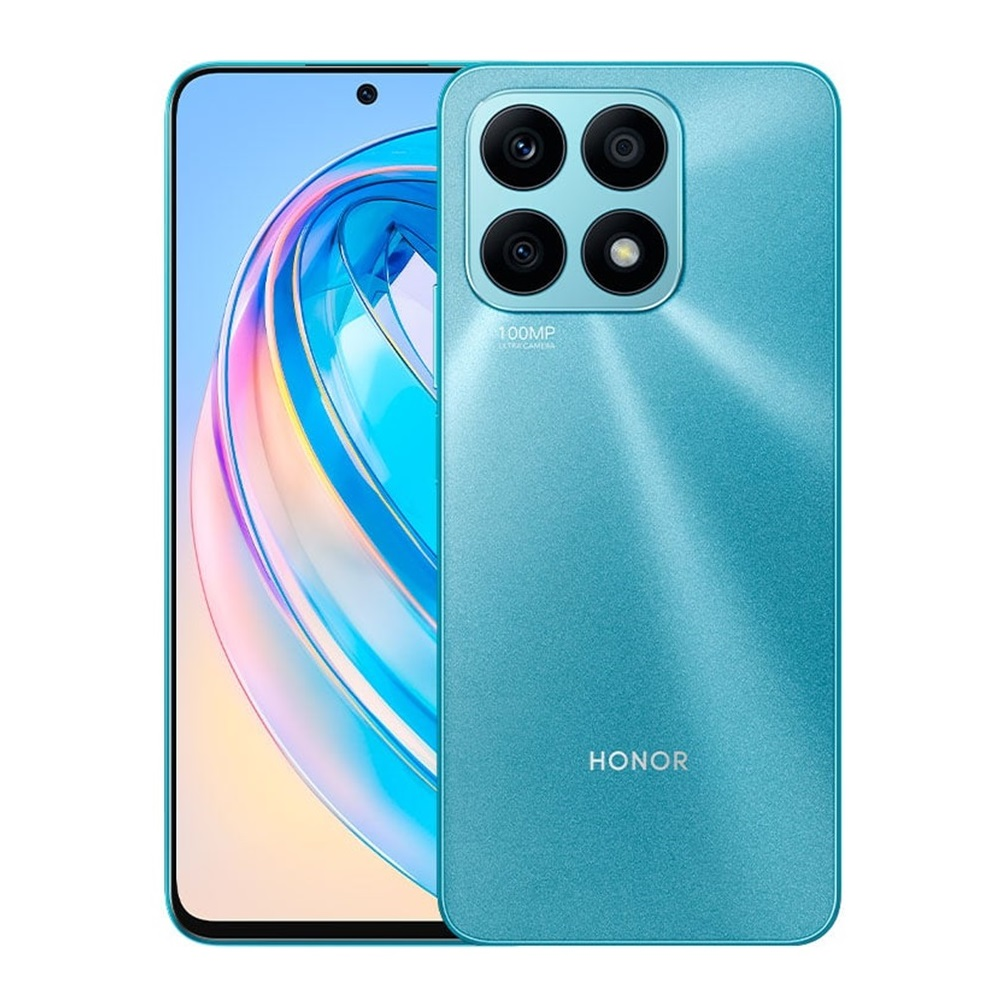
\includegraphics[width=.49\linewidth]{images/honor.jpg}
  \caption{Dispositivo movil Honor X8a utilizado para la toma de fotografias.}
  \label{fig:honor}
\end{figure}

\subsection{Proceso de Captura de Imágenes}

Se realizaron capturas de imágenes durante varias jornadas de trabajo en la obra, con el objetivo de obtener imágenes variadas de los trabajadores en diferentes situaciones, ángulos y posiciones. Las imágenes fueron tomadas en condiciones naturales de la obra, sin preparación previa de los trabajadores, con el fin de reflejar un entorno real. Se tomaron un total de 66 fotografías \ref{fig:photos} en distintas ubicaciones y con diferentes grupos de trabajadores, priorizando situaciones donde el uso de cascos de seguridad fuera evidente.

\begin{figure}[!ht]
  \centering
  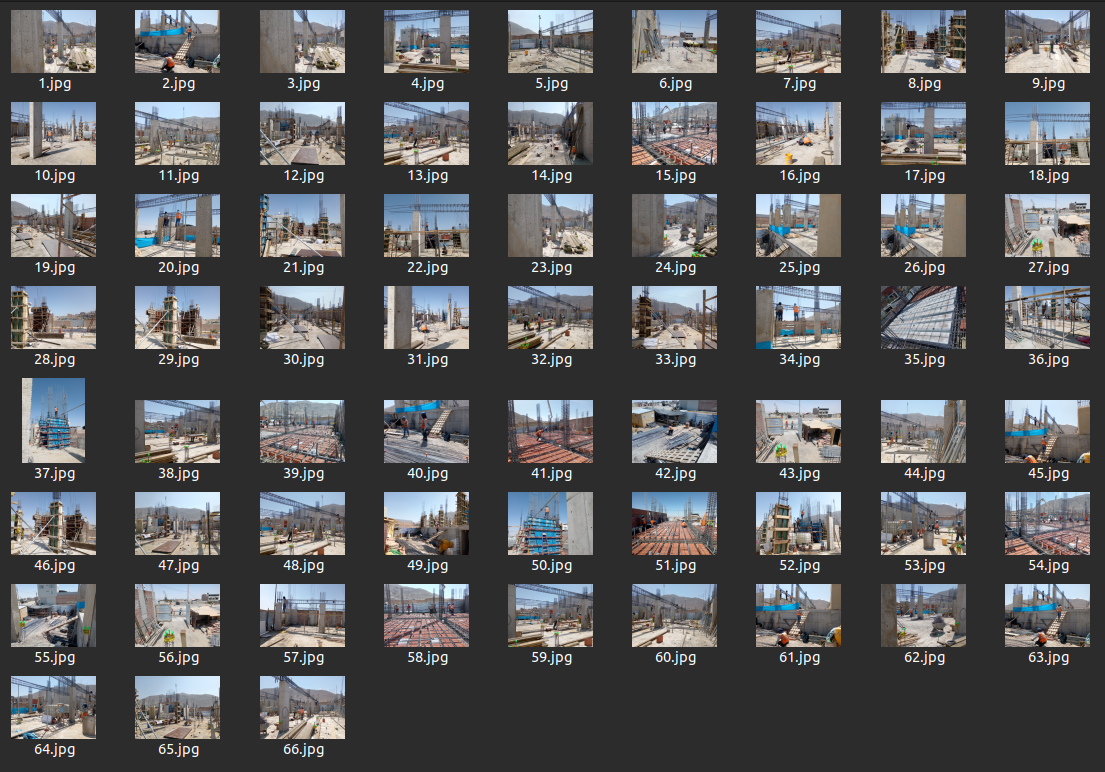
\includegraphics[width=.49\linewidth]{images/photos.png}
  \caption{66 fotografia tomadas en la obra ``Comercio''.}
  \label{fig:photos}
\end{figure}

\section{Preprocesamiento de los Datos}

\subsection{Redimensionamiento de Imágenes}

Las imágenes capturadas originalmente con una resolución de 5992x4344 píxeles fueron redimensionadas a 640x640 píxeles, que es el tamaño estándar requerido por el modelo YOLOv8 para su entrenamiento. Este proceso de redimensionamiento se llevó a cabo utilizando tres algoritmos diferentes de corte:

\begin{itemize}
  \item \textbf{Corte desde la izquierda:} Se inicia el recorte de las imágenes desde el borde superior izquierdo, generando múltiples imágenes de 640x640 píxeles hasta cubrir el área de la imagen original. Se deja un residuo en la parte final derecha con una dimension menor a 640 pixeles, de la misma manera en la parte inferior como se muestra en la figura \ref{fig:left_cropping}

\begin{figure}[!ht]
  \centering
  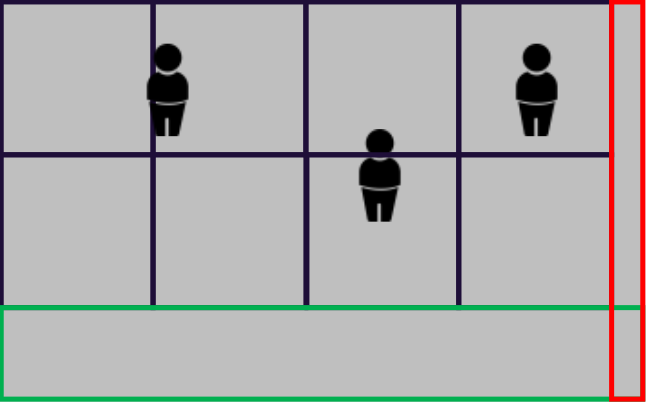
\includegraphics[width=.49\linewidth]{images/left_cropping.png}
  \caption{Esquema de recorte desde la izquierda.}
  \label{fig:left_cropping}
\end{figure}

\item \textbf{Corte centrado:} El recorte se realiza dividiendo el residuo de la imagen original entre los bordes izquierdo y derecho, así como entre el borde superior e inferior, para centrar la imagen de 640x640 píxeles en la escena como se muestra en la figura \ref{fig:center_cropping}.

\begin{figure}[!ht]
  \centering
  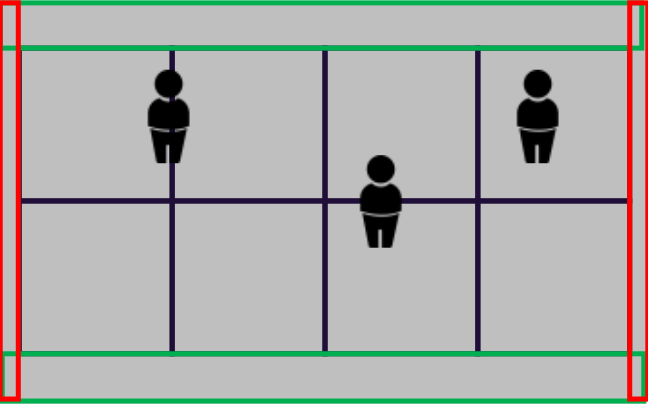
\includegraphics[width=.49\linewidth]{images/center_cropping.png}
  \caption{Esquema de corte centrado.}
  \label{fig:center_cropping}
\end{figure}

\item \textbf{Corte con superposición:} Se recortan imágenes de 640x640 píxeles con una pequeña porción de superposición entre ellas, generando imágenes adicionales para asegurar que todos los objetos presentes en la escena original estén representados como se muestra en la figura \ref{fig:full_cropping}.

\begin{figure}[!ht]
  \centering
  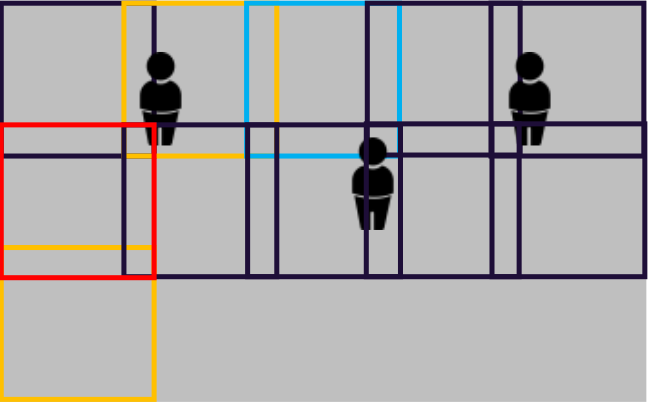
\includegraphics[width=.49\linewidth]{images/full_cropping.png}
  \caption{Esquema de corte con superposición.}
  \label{fig:full_cropping}
\end{figure}

\end{itemize}

\subsection{Filtrado de Imágenes}

Tras el proceso de recorte, no todas las imágenes contenían personas o trabajadores utilizando EPP. Para filtrar las imágenes sin relevancia, se utilizó un modelo YOLOv8m preentrenado, que detectó la presencia de personas en las imágenes recortadas. A aquellas imágenes que no contenían personas se les aplicó un filtro adicional con el modelo YOLOv8x, con un umbral de confianza del 90\%, para garantizar que las imágenes restantes contenían trabajadores en escenas donde el uso de cascos pudiera ser detectado. De esta manera, el dataset final se redujo a 642 imágenes útiles.

\subsection{Aumentación de Datos}

Para mejorar la generalización del modelo YOLOv8 durante el entrenamiento, se aplicaron técnicas de aumentación de datos utilizando la librería Keras. Se aplicaron las siguientes transformaciones a las imágenes:

\begin{itemize}
  \item \textbf{Rotación aleatoria (RandomRotation):}  Se rotaron las imágenes hasta un máximo del 10\% de 360 grados centrigrados, lo que introduce variabilidad en los ángulos de las imágenes.
  \item \textbf{Volteo horizontal (RandomFlip):} Se aplicó un volteo horizontal aleatorio a las imágenes.
\end{itemize}


\section{Etiquetado de Imágenes}

El etiquetado de las imágenes se llevó a cabo en la plataforma Roboflow como se muestra en la figura \ref{fig:roboflow_use}, una herramienta especializada para el etiquetado. Se creó un proyecto denominado ``helmet detection'', donde se cargaron las 1284 imágenes procesadas y aumentadas. Cada imagen fue revisada manualmente para etiquetar los cascos de seguridad, asignándoles la clase "helmet" en el formato compatible con YOLOv8.

\begin{figure}[!ht]
  \centering
  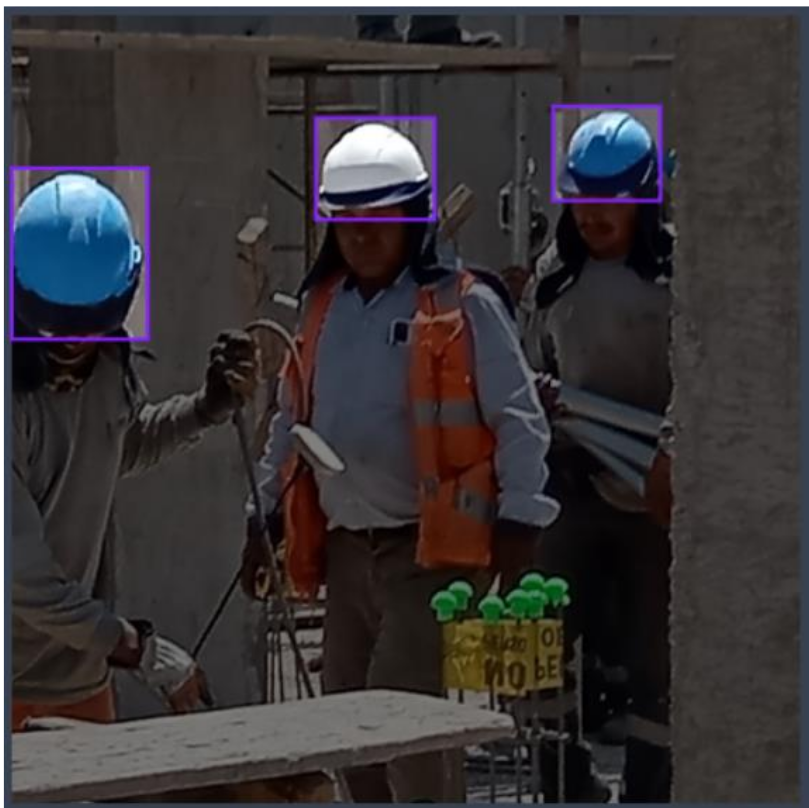
\includegraphics[width=.49\linewidth]{images/roboflow_use.png}
  \caption{Uso de la plataforma Roboflow para el etiquetado de la clase \textit{helmet}.}
  \label{fig:roboflow_use}
\end{figure}

